\documentclass[10pt]{article}
\usepackage[margin=17mm]{geometry}
\usepackage{graphicx,booktabs,hyperref}
\usepackage[strings]{underscore}
\setlength{\parindent}{0pt}\setlength{\parskip}{5pt}
\begin{document}
\section*{Qualified public queries: Boolean roots and actual points}

Native finite audit, 2026-10-25. All 2,048 planned rows are present in sixteen
128-query files. All finite-chain counts replay and all ordered signed point
counts independently agree in BinaryCurve/F2mElement arithmetic. The group
MITM combinatorial logic is shared, with separate exhaustive cyclic controls.
The independent arithmetic checks include lifts, actual bases, subgroup
membership, exact counts, witnesses and the predeclared selection.

\begin{center}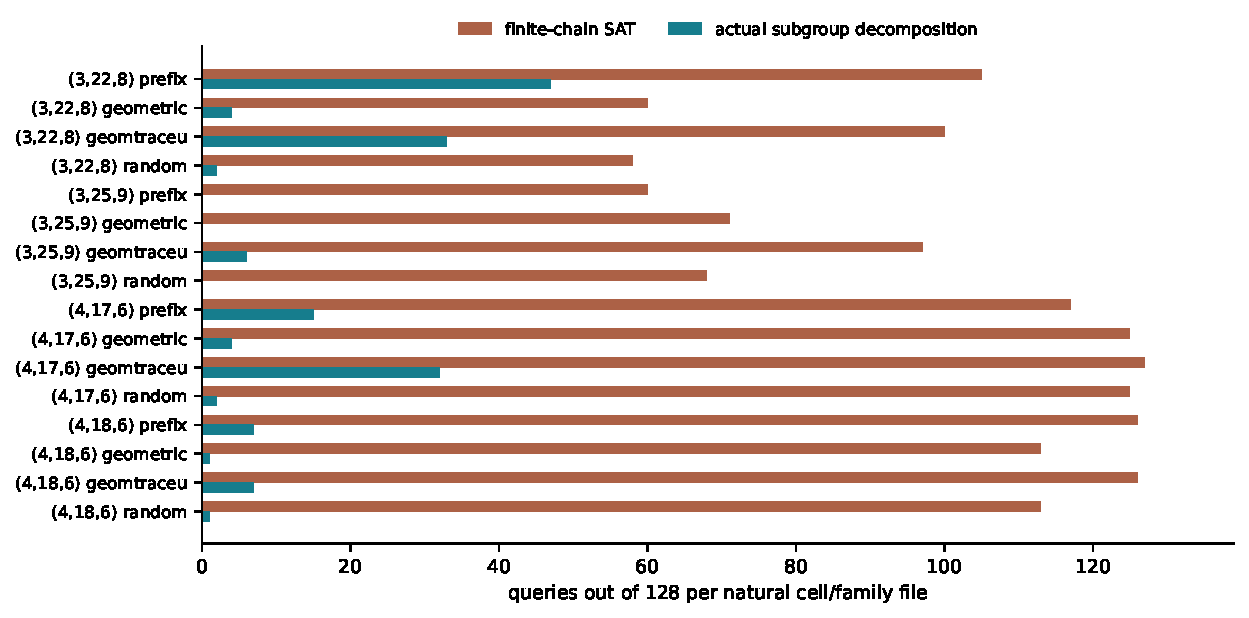
\includegraphics[width=\linewidth]{qualified-classes.pdf}\end{center}
\textbf{Observed:} 1,591 finite-chain SAT queries; 161 actual subgroup-SAT
queries, all among those 1,591. These are different output contracts. The
finite chain allows algebraic roots without an all-summands-in-G point relation
and has no infinity-intermediate variable. No identity between its root count
and the ordered signed point count is assumed. Empty bases and direct hits
remain in the full data, alongside quota shortages and duplicates.

\begin{center}\begin{tabular}{rrrrl}\toprule
n & b (integer) & Prime r & h & Curve-record SHA prefix\\\midrule
22 & 3159430 & 1048063 & 4 & \texttt{3b5cda776f80} \\
25 & 23461422 & 2096761 & 16 & \texttt{7424792732c8} \\
17 & 96838 & 16427 & 8 & \texttt{708752c13bf5} \\
18 & 102702 & 21821 & 12 & \texttt{a8f63491e295} \\
\bottomrule\end{tabular}\end{center}
All four selected models have a=0, full-field-degree b, exact factory point
counts, coprime r/h, and an explicitly checked nonzero generator of order r.
Target seed 202610250001: hash a curve identity and (m,n,ell,draw,attempt),
lift a uniform x, select a hashed sign, clear h, reject O and check rR=O.
The 512 underlying targets are paired across four families. Basis seed
202610250003 uses the separately frozen domain-separated encoding. No target
scalar is supplied by this constructor. Curve construction and each file
use 2-GiB/900-second caps; all generation and both replay streams exit zero.

Producer source 3cabc768f, frozen binary SHA prefix 9c38ff6e56ba; finite
replay binary prefix 4e7a01970e62; separate point-audit source a2c37d7bb.
Shared AMD EPYC 9V74 Linux x86-64 host, one Rayon thread, L0. Timings and
point-oracle operations are diagnostics, not complete query prices.

\textbf{Scope.} These are additional controls selected by an explicit a=0,
full-degree-b, cofactor-at-most-16 constructor rule, not a generic-curve
population result or a same-instance speed comparison with old b=1 fixtures.
No decomposition search cost, global minimum-guess law or complete DLP claim.
The original 1,159 reference/twist-audited fixtures remain unchanged.
Protocols: BINARY_QUERY_LAW_PROTOCOL.md and QUALIFIED_POINT_REPLAY_PROTOCOL.md.
Native receipt and all input hashes:
\path{../../pipeline-receipts/qualified-queries-20261025/summary.json}.
Raw tree is retained locally pending artifact-store upload; no upload claimed.

\end{document}
